\documentclass[../../TAU.tex]{subfiles}
\begin{document}

\chapter{Качество непрерывных систем управления}

\section{Показатели качества и типовые воздействия}

    Оказывается, рассмотренного ранее свойства устойчивости САУ недостаточно для описания качества его работы (точности, скорости и пр.). Например, в механических системах наличие колебаний (напр. качание деталей) ускоряет износ частей САУ, которые участвуют в этом движении. Устойчивость тоже иногда нуждается в оценке: насколько быстро система оказывается в заданном режиме.

    Наиболее полной характеристикой качества САУ является ошибка регулирования
    $$
        e(t) = g(t) - y(t).
    $$
    Зачастую при практической реализации есть определенные пожелания к виду (или поведению) этой функции, которые так или иначе могут быть сформулированы в виде математических выражений. Существует набор так называемых {\it показателей качества} --- это числовые показатели, характеризующие определенную часть работы системы. Эти показатели вычисляются {\bf только} для  устойчивых систем.

    \begin{figure}[h]
        \centering
        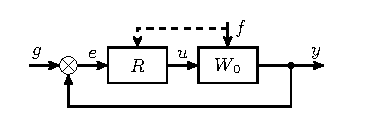
\includegraphics[width=8cm]{standard_system.pdf}
        \centering
        \caption{Типовая система}
        \label{FIG1}
    \end{figure}

    На рисунке~\ref{FIG1}: $W_0(s)$ --- ПФ объекта управления, $R(p)$ --- регулятор, $p=\frac{d}{dt}$, $f(t)$  --- возмущение.
    Имеем $y(t) = W_{yg}(p)g(t) + W_{yf}(p)f(t)$, где $W_{yf}(s)$ --- ПФ от возмущения к выходу. Тогда при задающем воздействии равном функции Хевисайда $\chi(t)$ ошибка имеет вид
    $$
    e(t) = W_{eg}(p) \chi(t) + W_{ef}(p) f(t),
    $$
    где $W_{eg}(p) = 1-W_{yg}$ --- ПФ от задающего воздействия к ошибке и $W_{ef} = - W_{yf}$ --- ПФ от возмущения к ошибке.

    В результате ошибка представима в виде
    $$
        e(t) = e_g(t) + e_f(t),
    $$
    где $e_g(t) = W_{eg}(p) g(t)$, $e_f(t) = W_{ef}(p) f(t)$. Показатели качества, естественно, исследуют отдельно по задающему воздействию и по возмущению.

    Еще одним аспектом различения показателей качества является режим работы САУ. Выделяют переходный режим и установившийся режим.
    Из курса ОДУ известно, что выход системы можно представить в виде
    $$
        y(t) = y_{св}(t) + y_{вын}(t),
    $$
    на которое опирается введение терминов в ТАУ
    $$
        y(t) = y_{пр}(t) + y_{\infty}(t),
    $$
    где $y_{пр}(t)$ содержит в себе, как слагаемые,  $y_{св}(t)$ и часть из $y_{вын}(t)$, $y_{\infty}(t)$ целиком содержится в $y_{вын}(t)$.

    \textit{Комментарий.} Понять последнее удобнее всего на ОДУ, например, второго порядка с правой частью равной $1$. Тогда $y_{\infty}(t)=\const$, а все остальное в решении будет переходной составляющей $y_{пр}(t)$. Если входное воздействие не константа, а гармонический сигнал, входное решение ОДУ
    также может быть разбито на составляющие без особого труда, если вспомнить о свойствах линейного звена при прохождении сквозь него гармонического сигнала.

    {\it Показатели качества в переходном режиме} строятся при {\it типовом внешнем воздействии} $g(t) = A\cdot\chi(t)$ --- функция Хевисайда, где $A=\const$. Обычно полагают $A=1$.

    {\it Показатели качества в установившемся режиме} строятся при типовых воздействиях вида $A\cdot\chi(t),\; At,\; At^2,\; \ldots$.

    И те и другие показатели рассматриваются при нулевых начальных условиях. Перейдем к рассмотрению показателей качества в переходном режиме.

\subsection{Прямые показатели качества}

    Ошибка при ступенчатом воздействии (step response) имеет вид
    $$
        e(t) = 1(t) - h(t),
    $$
    где $h(t)$ --- переходная функция. Из-за простой связи $h(t)$ и $e(t)$ показатели качества определяют по $h(t)$.
    \begin{defi}
        Прямыми показателями качества называются показатели, определяемые непосредственно по переходной характеристике.
    \end{defi}

    \begin{figure}[h]
        \centering
        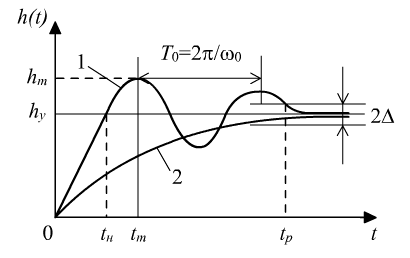
\includegraphics[width=8cm]{step_response.png}
        \centering
        \caption{Переходная функция системы}
        \label{FIG2}
    \end{figure}

    Определения показателей качества в переходном режиме:
    \begin{enumerate}
        \item {\it Временем регулирования $t_\text{р}$}
            называется время, за которое значение переходной функции $h(t)$ входит в $\delta$-трубку и не выходит из неё, т.е. $|h(t)-h_{\infty}| <\delta $ при $t \ge t_\text{p}$, где $h_\infty = \lim\limits_{t\rightarrow\infty} h(t)$, $\delta$ --- заданное число, которое обычно полагают 5-10\% от $|h_{\infty}|$;
        \item {\it Временем нарастания $t_\text{н}$}
            называется время, через которое значение переходной функции впервые становится равным $h_\infty$;
        \item {\it Перерегулированием $\sigma$}
            называют число, равное
            $$
                \sigma = \left|\frac{h_m-h_\infty}{h_\infty}\right|\cdot100\%,
            $$
            где $h_m$ --- максимальное значение, принимаемое $h(t)$.

            В частности, возможно, что $h_\infty = 0$, тогда перерегулирование определяется формулой $ \sigma = \frac{y_m}{A}\cdot 100\%$, где $y_m$ --- максимальное значение выхода при возмущении $f(t) = A\cdot\chi(t)$;
        \item {\it Числом колебаний $N_\text{к}$} 
            называют количество полных колебаний $h(t)$ за время регулирования.
    \end{enumerate}

\subsection{Косвенные показатели качества (корневые)}

    {\it Косвенными показателями качества} называются показатели, определяемые не по переходной функции.

    К {\it корневым показателям} качества относят {\it степень колебательности $\mu$} и {\it степень устойчивости $\eta$}:
    \begin{enumerate}
        \item 
            $\eta=\min\limits_{j}|\RE s_j| = -\max\limits_j \RE s_j$, где $s_j$ --- корни характеристического полинома САУ;\\
            \begin{center}
            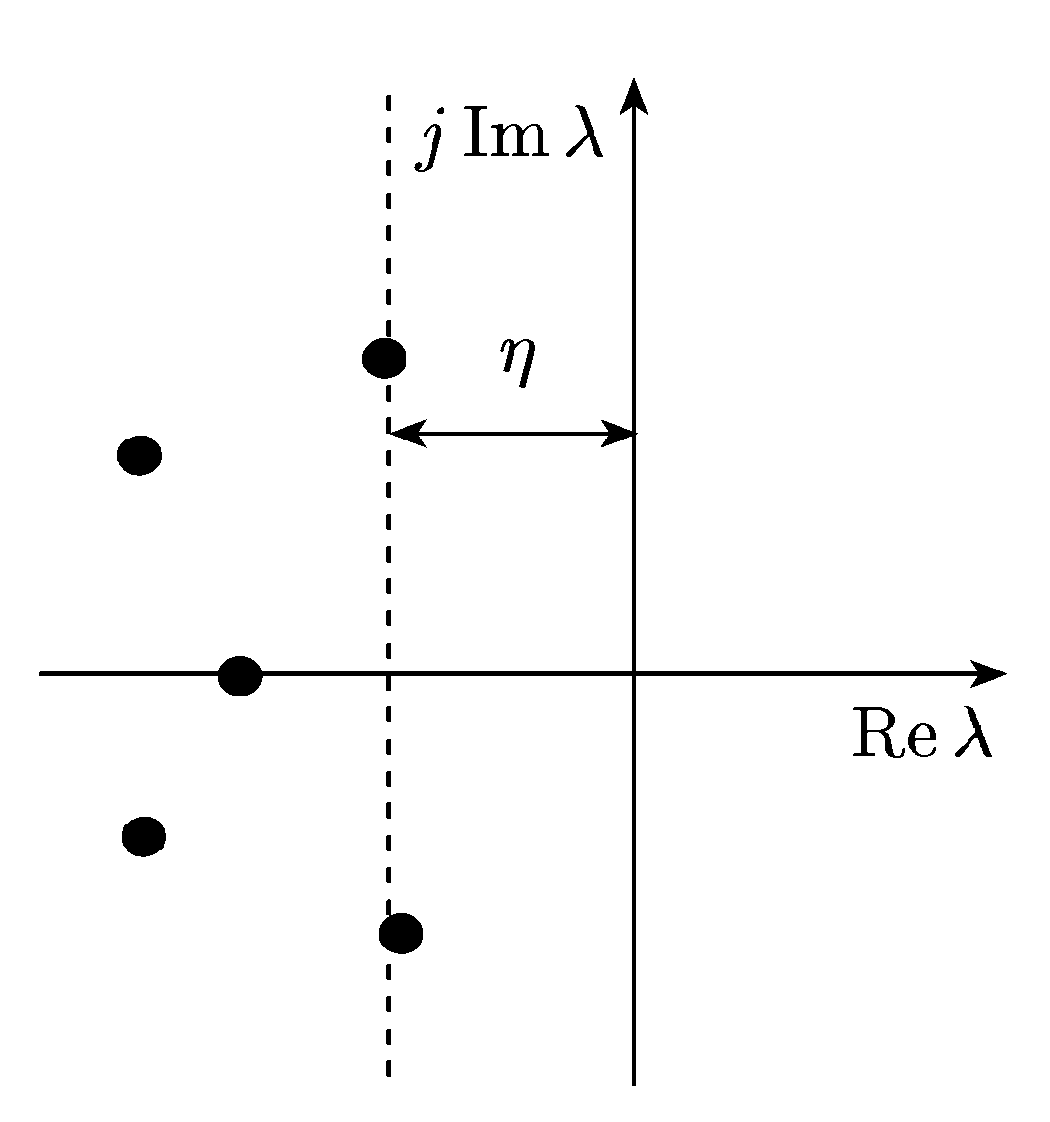
\includegraphics[height=43mm]{stable_prop.png}
            \end{center}

            \begin{figure}[h]
                \centering
                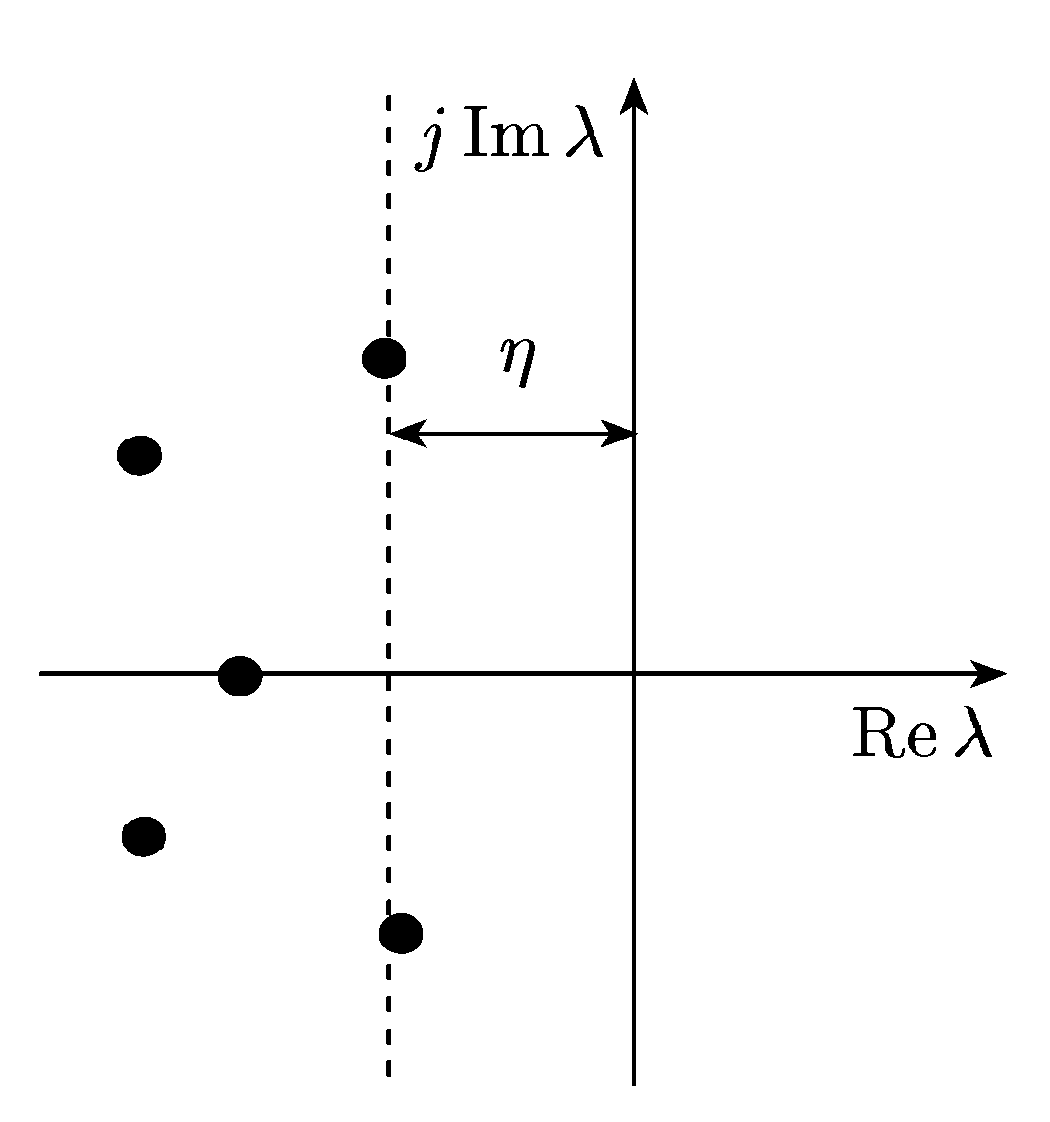
\includegraphics[width=4.3cm]{stable_prop.png}
                \caption{Статическая характеристика П-звена}
                \centering
            \end{figure}
        \item 
            $\mu = \max\limits_j\left|\frac{\IM s_j}{\RE s_j}\right| = \max\limits_j tg\phi_j$, где $\phi_j$ --- угол наклона вектора с концом в корне $s_j$ к отрицательному направлению вещественной оси.
            \begin{center}
            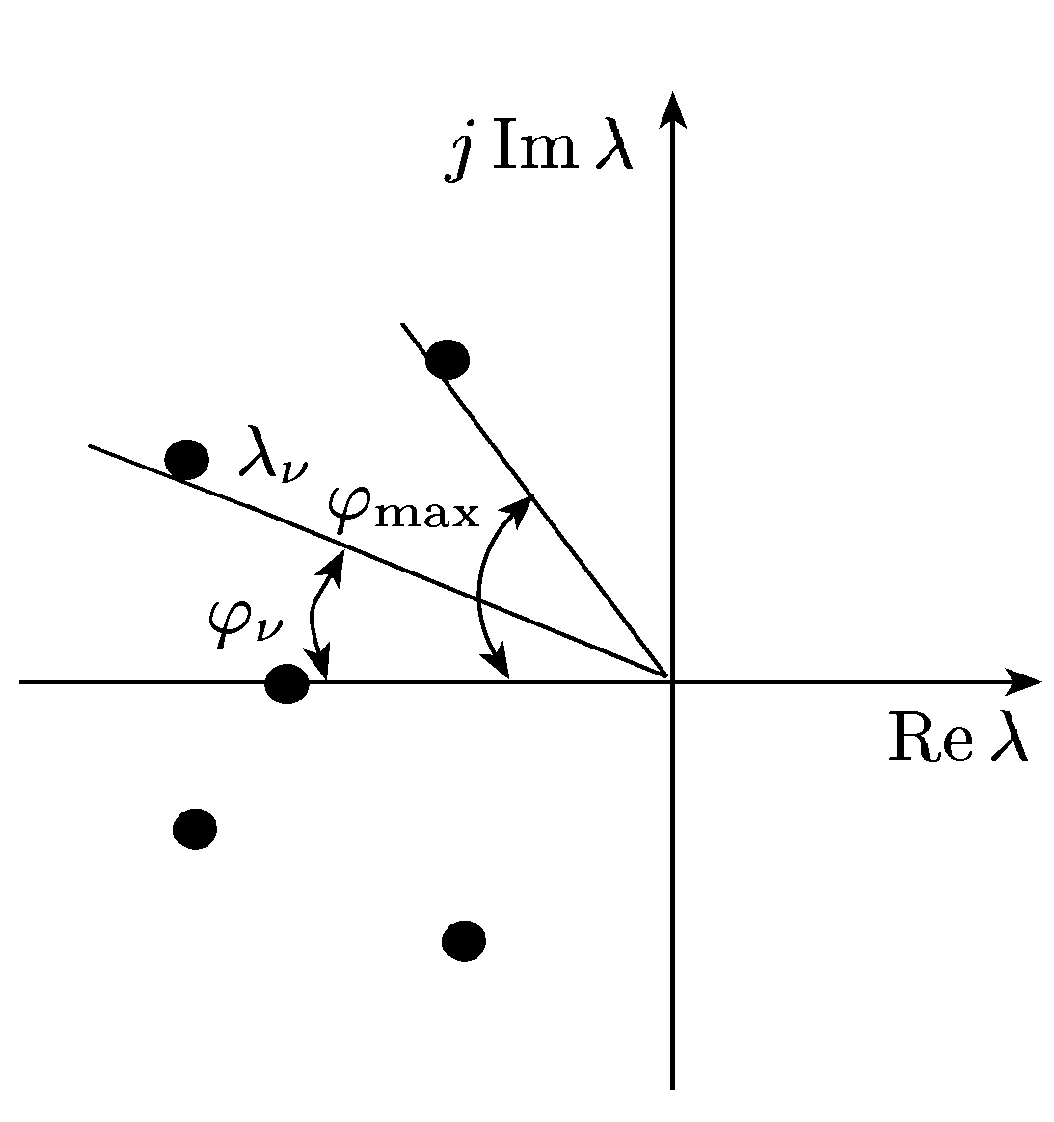
\includegraphics[height=50mm]{oscilate_prop.png}
            \end{center}
    \end{enumerate}

\subsection{Степень устойчивости}

    Как определить степень устойчивости $\eta$, не находя корней? Обычно этот вопрос упрощают до вопроса сравнения данного положительного числа $c$ с $\eta$. Сравнение же можно выполнить, не вычисляя  корней полинома.

    Рассмотрим полином $\tilde\gamma(s) = \gamma(s-c)$. Корни полинома $\tilde\gamma(s)$ сдвинуты вправо относительно корней $\gamma(s)$ ровно на $c$. Если полином $\tilde\gamma(s)$ остался устойчивым, тогда, очевидно, $\eta > c$ в противном случае $\eta \le c$.

    Пусть $\tilde\gamma(s) = s^n + \tilde\gamma_{n-1}s^{n-1} + \ldots + \tilde\gamma_1 s + \tilde\gamma_0.$

    Тогда
    $$
        \left.\frac{d^i \tilde\gamma}{ds^i}\right|_{s=0} = i!\tilde\gamma_i,\; i=\cnt{0,n-1}.
    $$
    С другой стороны $\left.\frac{d^i \tilde\gamma}{ds^i}\right|_{s=0} = \left.\frac{d^i \gamma(s-c)}{ds^i}\right|_{s=0}=\left.\frac{d^i \gamma(s)}{ds^i}\right|_{s=-c}$. Поэтому имеем
    $$
        \tilde\gamma_i = \frac{1}{i!}\left.\frac{d^i \gamma(s)}{ds^i}\right|_{s=-c}.
    $$

    \examp{Пусть $\gamma(s) = s^4+2s^3+5s^2+3s+1$. Сравнить степень устойчивости данного полинома с $c=0.5$.}

\subsection{Показатели качества в переходном режиме. Косвенные показатели качества (интегральные)}

    Представим ошибку в виде
    $$
        e(t) = e_\text{п}(t)+e_{\infty}(t),
    $$
    где $e_\text{п}(t)$ и $e_{\infty}(t)$ --- переходная и установившаяся составляющие ошибки. Так как в данном случае типовое воздействие $g(t)\equiv\chi(t)$, то $e_\infty(t) = \const = 1-h_\infty$.

    Рассмотрим функционал $J_{20} = \int\limits_{0}^{\infty}e_\text{п}^2(t)dt$. Это число называется {\it интегральной квадратической ошибкой} (оценкой), оно характеризует стремление ошибки $e_{\text{п}}(t)$ к нулю, в частности, из $J_{20}\rightarrow0$ следует $\max\limits_{t\in[0,\infty]}|e_{\text{n}}(t)|\rightarrow0$.

    Однако, даже при малой оценке $J_{20}$ возможно, что переходный процесс будет колебательным, поэтому используют {\it обобщенные интегральные квадратические оценки}.

\section{Интегральные показатели качества }

    {\it Обобщенными интегральными квадратическими оценками} называют функционалы  вида
    $$
        J_{2k} = \int\limits_0^\infty\left[e_\text{п}^2(t)+\tau^2_1\dot e_\text{п}^2(t) + \ldots + \tau^2_k \stackrel{(k)} {e_\text{п}}\vphantom{e_\text{п}}^2(t)\right]dt,
    $$
    где $\tau_i$ --- некоторые числа, определяемые в зависимости от требований качества САУ. Смысл этих параметров виден из следующего.

    Нетрудно представить $J_{21} = \int\limits_0^\infty\left[e_\text{п}^2(t) + \tau^2\dot e^2_\text{п}(t)\right]dt$ в виде
    $$
        J_{21} = \int\limits_0^\infty\left[e_\text{п}(t) +\tau\dot e_\text{п}(t)\right]^2dt -2\tau \int\limits_0^\infty e_\text{п}(t)\dot e_\text{п}(t) dt,
    $$
    где нетрудно видеть $\int\limits_0^\infty e_\text{п}(t)\dot e_\text{п}(t) dt = -\frac{1}{2}e_\text{п}^2(0)$.

    Откуда получим, что
    $$
        J_{21} = \int\limits_0^\infty\left[e_\text{п}(t) +\tau\dot e_\text{п}(t)\right]^2dt + \tau e^2_\text{п}(0).
    $$

    Таким образом, минимум функционала $J_{21}$ достигается при $e_\text{п}(t)$, удовлетворяющем уравнению
    $$
        \tau\dot e_\text{п}(t) + e_\text{п}(t) = 0.
    $$

    Можно аналогично получить, что $J_{2k}$ достигает минимума, если выполнено уравнение
    $$
        \tau_k \stackrel{(k)}{e_\text{п}} (t) + \ldots + \tau_1 \dot e_\text{п}(t) + e_\text{п}(t) = 0.
    $$




\subsection{Вычисление интегральных показателей качества}

    Для вычисления интегральных оценок удобно использовать равенство Парсеваля
    $$
        \int\limits_0^\infty x^2(t) dt = \frac{1}{2\pi} \int\limits_{-\infty}^{\infty} |X(i\omega)|^2 d\omega.
    $$
    Тогда
    $$
        \begin{aligned}
            J_{20} &= \frac{1}{2\pi}\int\limits_{-\infty}^{\infty}|E_\text{п}(i\omega)|^2d\omega\\
            J_{2k} &= \frac{1}{2\pi}\int\limits_{-\infty}^{\infty}|E_\text{п}(i\omega)|^2 + \tau_1^2 |\dot E_\text{п}(i\omega)|^2 + \ldots \tau_k^2 |\stackrel{(k)}{E_\text{п}}(i\omega)\vphantom{E(i\omega)}|^2 d\omega,
        \end{aligned}
    $$
    где $E_\text{п}(s) = L\{e_\text{п}(t)\}$, $\dot E_\text{п}(s) = L\{\dot e_\text{п}(t)\}$, \ldots.

    Так как $\dot E_\text{п}(s) = sE_\text{п}(s) - e_\text{п}(0)$, то
    $$
        J_{21} = J_{20} + \frac{\tau^2}{2\pi}\int\limits_{-\infty}^\infty\left|i\omega E_\text{п}(i\omega) - e_\text{п}(0)\right|^2 d\omega,
    $$
    где $e_\text{п}(0)$ находится из свойства преобразования Лапласа $e_\text{п}(0) = \lim\limits_{s\rightarrow\infty}sE_\text{п}(s)$.

    Таким образом, вычисление этих оценок связано с вычислением интегралов вида
    $$
        I_n = \frac{1}{2\pi}\int\limits_{-\infty}^\infty \left|\frac{b_{n-1}(i\omega)^{n-1} + \ldots + b_1 i\omega + b_0}{a_{n}(i\omega)^{n} + \ldots + a_1 i\omega + a_0}\right|^2d\omega,
    $$
    которые вычисляются с помощью вычетов ТФКП.

    Частные случаи:
    \begin{center}
    $$
        \begin{aligned}
            n=1:\qquad  &I_1 = \frac{b_0^2}{2a_1a_0};\\
            n=2:\qquad  &I_2 = \frac{b_0^2a_2 + b_1^2a_0}{2a_2a_1a_0};\\
            n=3:\qquad &I_3 = \frac{b_0^2a_2a_3 + (b_1^2-2b_0b_2)a_0a_3 + b_2^2a_0a_1}{2a_3a_0(a_1a_2-a_0a_3)}.
        \end{aligned}
    $$
    \end{center}

    \examp{Вычислить среднеквадратические ошибки $J_{20}$ и $J_{21}$ для системы с ПФ $W(s) = \frac{3}{0.1s+1}$, $g=\chi(t)$ и $f=0$.
        \begin{figure}[h]
            \centering
            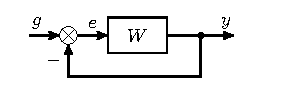
\includegraphics[width=8cm]{system_for_int_e.pdf}
        \end{figure}}

\section{Установившийся режим}

\subsection{Показатели качества в установившемся режиме }

    Вспомним, что в {\it установившемся режиме} рассматриваются типовые воздействия вида $A,At, At^2, \ldots$. Тогда в представлении ошибки по задающему воздействию, например, имеем
    $$
        e_g(t) = e_{gп}(t) + e_{g\infty}(t),
    $$
    где интересующая нас функция $e_{g\infty}(t)$ такова, что для воздействий $At, At^2, \ldots$ не существует конечного предела $\lim\limits_{t\rightarrow\infty} e_{g\infty}(t)$. Это связано с тем, что задающее воздействие $g(t)$ растущая функция. В частности, если выполнено $\lim\limits_{t\rightarrow\infty} e_{g\infty}(t)=0$ для $g(t) = At^r$ и не выполнено для $g(t) = At^{r+1}$, тогда говорят, что система обладает $r$-м порядком астатизма, т.е. система в установившемся режиме не реагирует (инвариантна) к таким воздействиям.

    Сказанное выше также относится и к ошибке по возмущению $e_f(t)$.

\subsection{Коэффициенты ошибок в установившемся режиме}

    ПФ $W_{eg}(s) $ устойчивой системы можно разложить в ряд Тейлора в правой комплексной полуплоскости
    $$
        W_{eg}(s) = W_{eg}(0) + \frac{1}{1!}\left.\frac{dW_{eg}(s)}{ds}\right|_{s=0}s + \frac{1}{2!}\left.\frac{d^2W_{eg}(s)}{{ds}^2}\right|_{s=0}s^2 + \ldots
    $$
    в силу аналитичности функции $W_{eg}(s)$ в некоторой области, содержащей правую полуплоскость с границей (место для медитации). Тогда из равенства
    $$
        E_g(s) = W_{eg}(s) G(s),
    $$
    получим (место для медитации)
    $$
        e_{g\infty}(t) = C_{g0} g(t) + C_{g1} \dot g(t) + C_{g2} \ddot g(t) + \ldots,
    $$
    где $C_{gi} =\frac{1}{i!}\left.\frac{d^iW_{eg}(s)}{ds^i}\right|_{s=0}$, $i=0,\;1,\;2,\;\ldots$.

    Аналогичное представление верно и для ошибки по возмущению:
    $$
        e_{f\infty}(t) = C_{f0} f(t) + C_{f1} \dot f(t) + C_{f2} \ddot f(t) + \ldots,
    $$
    где $C_{fi} =\frac{1}{i!}\left.\frac{d^iW_{ef}(s)}{ds^i}\right|_{s=0}$, $i=0,\;1,\;2,\;\ldots$.

    Первые три ошибки имеют свои имена
    \begin{enumerate}
        \item $C_{g0},\; C_{f0}$ --- коэффициенты позиционной ошибки (по воздействию и возмущению)
        \item $C_{g1},\; C_{f1}$ --- коэффициенты ошибки по скорости (по воздействию и возмущению)
        \item $C_{g2},\; C_{f2}$ --- коэффициенты ошибки по ускорению (по воздействию и возмущению)
    \end{enumerate}

    \begin{defi}
    Статической ошибкой называют установившуюся ошибку при единичном ($g(t) = \chi(t)$) входном воздействии.
    \end{defi}

    \begin{defi}
    САУ называют статической, если её статическая ошибка отлична от нуля.
    \end{defi}

    \begin{defi}
    САУ называют астатической, если её статическая ошибка равна нулю.
    \end{defi}

    \begin{defi}
    Говорят, что САУ имеет $r$-ый порядок астатизма (по возмущению/воздействию), если если первые $r$ коэффициентов ошибок равны нулю, а $r+1$ --- не равен.
    \end{defi}

\section{Астатическая САУ}

    Пусть система обладает $r$-м порядком астатизма по воздействию. Тогда при воздействии $g(t) = a_0+a_1t+\ldots+ a_{r-1}t^{r-1}$ ошибка равна $e_{g\infty}(t) = 0$. А для воздействия $g(t) = a_0+a_1t+\ldots+ a_{r}t^{r}$ имеем ошибку $e_{g\infty}(t) = \const$.

    Кроме того, для такой системы можно вычислять коэффициенты ошибок по формуле
    $$
        C_{gi} = \left.\frac{W_{eg}(s)}{s^i}\right|_{s=0},
    $$
    где $i = \cnt{0,r}$. Аналогично для коэффициентов по возмущению.

\subsection{Структура астатической по воздействию САУ }

    Рассмотрим подробнее систему с $r$-м порядком астатизма {\it по воздействию} со следующей структурной схемой:
    \begin{figure}[h]
        \centering
        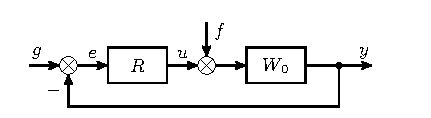
\includegraphics[width=8cm]{astatic_system.pdf}
    \end{figure}

    Тогда $W_{eg}(s) = s^r\bar W_{eg}(s)$, где $\bar W_{eg}(s) = \frac{q(s)}{p(s)}$ и $q(0)\neq 0$.

    ПФ прямой цепи $W(s) = W_0(s)R(s)$, где $W_0(s) = \frac{\beta(s)}{\alpha(s)}$, $R(s) = \frac{\phi(s)}{\psi(s)}$. Из структурной схемы имеем
    $$
        W_{eg}(s) = \frac{1}{1+W_0R} = \frac{\alpha\psi}{\alpha\psi+\beta\phi}
    $$
    откуда следует, что $\alpha(s)\psi(s) = s^r q(s)$.

\subsection{Структура астатической по возмущению САУ }

    Рассмотрим подробнее систему с $r$-м порядком астатизма {\it по возмущению} со следующей структурной схемой:
    \begin{figure}[h]
        \centering
        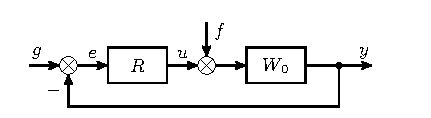
\includegraphics[width=8cm]{astatic_system.pdf}
    \end{figure}

    Тогда $W_{ef}(s) = s^r\bar W_{ef}(s)$, где $\bar W_{ef}(s) = \frac{h(s)}{k(s)}$ и $h(0)\neq 0$.

    По аналогии с предыдущим случаем получим
    $$
        W_{ef}(s) = -\frac{W_0}{1+W_0R} = -\frac{\beta\psi}{\alpha\psi+\beta\phi}
    $$
    откуда следует, что $\beta(s)\psi(s) = -s^r h(s)$.

    \examp{Даны ОУ и регулятор с ПФ вида
    $$
    W_0(s) = \frac{4}{s(s+1)},\qquad R(s) = \frac{5s+1}{10s}.
    $$
    Задающее воздействие и возмущение имеют вид $g(t) = 1+0.1t$ и $f(t) = 0.2+0.2t$. Определить установившиеся ошибки $e_{g\infty}(t)$ и $e_{f\infty}(t)$, если система описывается структурной схемой
    \begin{figure}[h]
        \centering
        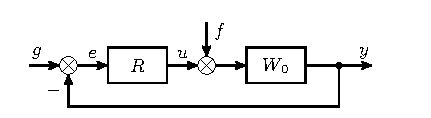
\includegraphics[width=8cm]{astatic_system.pdf}
    \end{figure}
    }

\section{Синтез САУ с заданным качеством. Пример}

    \examp{Для системы, изображенной на структурной схеме с $W(s) = \frac{10}{s(s+10)}$, синтезировать регулятор $R(s)=k$ (П-регулятор), чтобы степень колебательности $\mu$ системы была равна нулю и интегральная ошибка $J_{21}$ при $\tau=0.5$ была минимальна.
    \begin{figure}[h]
        \centering
        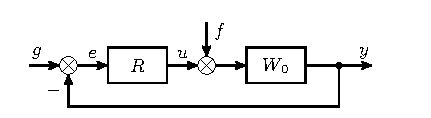
\includegraphics[width=8cm]{astatic_system.pdf}
    \end{figure}
    }

\section{Синтез САУ по желаемой передаточной функции}

    Во многих случаях синтез САУ с заданным качеством можно свести к синтезу САУ по желаемой передаточной функции $\tilde W(s)$. Тогда первым шагом производится выбор передаточной функции, которая удовлетворяет требуемому качеству, а затем производится синтез САУ по желаемой ПФ.

    Общие требования к замкнутой системе:
    \begin{enumerate}
        \item 
            физическая реализуемость $R(s)$ и строгая ф.р. $\tilde W(s)$ ;
        \item 
            порядок ПФ $\tilde W(s)$ не меньше ПФ $W(s)$;
        \item 
            грубость относительно свойства устойчивости, т.е. устойчивость при малой вариации параметров системы сохраняется.
    \end{enumerate}
    Рассмотрим следующие требования к качеству САУ:
    \begin{enumerate}
      \item требование к степени устойчивости: $\eta > c=\const$;
      \item апериодичность переходного процесса;
      \item порядок астатизма равен $r$ (по воздействию и по возмущению).
    \end{enumerate}

\subsection{Постановка задачи}

    \begin{figure}[h]
        \centering
        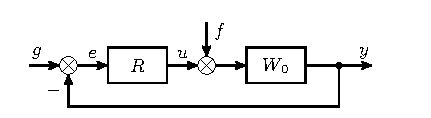
\includegraphics[width=8cm]{astatic_system.pdf}
    \end{figure}

    Нетрудно вычислить ПФ замкнутой системы:
    \begin{equation}\label{WYG}
        W_{yg}(s) = \frac{RW_0}{1+RW_0}.
    \end{equation}

    Задача. Требуется найти $R$ такой, что $W_{yg}(s) = \tilde W (s)$ --- желаемая ПФ, удовлетворяющая общим требованиям и требованиям к качеству.

    Требования к апериодичности и степени устойчивости системы, а также общее требование $2$ на порядок разрешаются выбором знаменателя $\tilde W(s) = \frac{\xi(s)}{\gamma(s)}$. Будем считать, что $\gamma(s)$ выбран.

\subsection{Исследование}

    Из \eref{WYG} следует, что
    $$
        \tilde W(1+RW_0) = RW_0 \Longrightarrow R = \frac{1}{W_0}\frac{\tilde W}{1-\tilde W}.
    $$

    Выполнение пункта 3 общих требований в данном случае связано с сокращением неустойчивых нулей и полюсов регулятора и ОУ. Действительно, представим $W_0(s) = \frac{\beta(s)}{\alpha(s)} = \frac{\beta^-(s)\beta^+(s)}{\alpha^-(s)\alpha^+(s)}$, где знаки $-$ и $+$ означают устойчивость и неустойчивость корней полиномов. Тогда
    $$
        R(s) = \frac{\alpha^-(s)\alpha^+(s)}{\beta^-(s)\beta^+(s)}\frac{\tilde W}{1-\tilde W}.
    $$

    Чтобы сокращений не было, потребуем
    $$
        \tilde W(s) = \frac{\beta^+(s)M(s)}{\gamma(s)}\quad \text{и}\quad 1-\tilde W(s) = \frac{\alpha^+(s)N(s)}{\gamma(s)}.
    $$

    Система будет иметь $r$-й порядок астатизма по воздействию, если в контуре замкнутой системы расположены $r$ интегрирующих звеньев, т.е. совокупно в знаменателях регулятора и ОУ содержится $s^r$. Учтем, что исходная система может давать вклад в порядок астатизма, если  $\alpha^+(s) = s^{k_\alpha} \alpha^*(s)$, где $\alpha^*(0)\neq0$. Тогда положив
    \begin{equation}\label{EQ1}
        1-\tilde W(s) = \frac{\alpha^+(s)s^{l_g}N(s)}{\gamma(s)},
    \end{equation}
    где $l_g = r-k_\alpha$, удовлетворим требованию астатизма по воздействию.

    Заметим, что
    $$
        W_{ef}(s) = \frac{W}{1+WR} = \frac{\beta\psi}{\alpha\psi+\beta\phi},
    $$
    где $\psi$ --- знаменатель $R(s)$. Очевидно, что астатизм $r$-го порядка по возмущению $f$ достигается, если знаменатель $R(s)$ содержит член $s^{l_f}=s^{r-k_\beta}$, где $k_\beta:\; \beta(s) = s^{k_\beta}\beta^*(s),\; \beta^*(0)\neq0$. Таким образом, заменив $l_g$ на $l=\max\{l_g,\;l_f\}$ в \eref{EQ1} удовлетворим всем требованиям качества.

    Определим вид полученного регулятора. Сложив два выражения
    $$
        \tilde W(s) = \frac{\beta^+(s)M(s)}{\gamma(s)}\quad \text{и}\quad 1-\tilde W(s) = \frac{\alpha^+(s)s^lN(s)}{\gamma(s)},
    $$
    получим
    $$
        1 = \frac{\beta^+(s)M(s)+\alpha^+(s)s^lN(s)}{\gamma(s)},
    $$
    откуда
    \begin{equation}\label{EQ2}
        \gamma(s) = \beta^+(s)M(s)+\alpha^+(s)s^lN(s).
    \end{equation}
    В последнем уравнении необходимо подобрать полиномы $M(s)$ и $N(s)$, а точнее определить степени, при которых такие полиномы найдутся.
%Остается разрешить вопрос о физической реализуемости $R(s)$.
    Обозначим $\deg\alpha^+ = n_{\alpha+},\; \deg\beta^+ = n_{\beta+},\; \deg M = n_M,\; \deg N = n_N,\; \deg\gamma = n_\gamma, \deg\beta=n_{\beta},\deg\alpha=n_{\alpha}$. Для разрешимости \eref{EQ2} достаточно потребовать, чтобы число неизвестных ($n_M+n_N+2$) было больше числа уравнений ($n_\gamma+1$):
    $$
        \boxed{n_\gamma-1 \le n_M+n_N}.
    $$

    Для выполнения требования физической осуществимости $R(s)$ вида
    $$
        R(s) = \frac{\alpha^-(s)\alpha^+(s)}{\beta^-(s)\beta^+(s)}\frac{\tilde W}{1-\tilde W}
    $$
    достаточно, чтобы было выполнено неравенство
    $$
        \begin{aligned}
            n_{\alpha}+n_{\beta+}+n_M \le n_{\beta}+l+n_{\alpha+}+n_N\Longrightarrow\\
            \boxed{n_M-n_N \le n_{\beta}-n_{\beta+}-(n_{\alpha}-n_{\alpha+}) + l}.
        \end{aligned}
    $$

    Строгая физическая реализуемость $\tilde W(s)$ достигается только тогда, когда степень числителя меньше степени знаменателя,т.е.
    $$
        \boxed{n_\gamma > n_{\beta+}+n_M}.
    $$
    Условие
    $$
        1-\tilde W(s) = \frac{\alpha^+(s)s^lN(s)}{\gamma(s)}
    $$
    выполнено, только если выполнено равенство
    $$
        \boxed{n_\gamma = n_{\alpha+}+l+n_N}.
    $$

    \examp{ПФ ОУ имеет вид $W(s) = \frac{1}{s(s+1)}$. Требования:
        \begin{enumerate}
          \item $e_\text{п}(t) = (C_1+C_2t+C_3t^2)e^{-t}$
          \item $e_{g\infty} = 0, \text{при } g=\const$
          \item $e_{f\infty} = 0, \text{при } f=\const$
        \end{enumerate}
    }




\end{document}